\documentclass{SNJB}
\usepackage{babel}
\usepackage{babel}
\usepackage{algorithm}
\usepackage{algorithmic}

\usepackage{caption}
\usepackage{amssymb}
\usepackage{amsmath}
\usepackage{subfigure}
\usepackage{graphicx}
\usepackage{fancybox}

\usepackage{url}
\usepackage[breaklinks=true]{hyperref}

\usepackage[]{nomencl}
\renewcommand{\nomname}{Abbreviations}
\makenomenclature

\makeindex

\begin{document}

\title{Smart Bus System}
\author{Sharma Sagar Ganesh}

\newauthor{prof.Y.K.Desai}

\new{Name: Sharma Sagar Ganesh  \\ \new{1.5cm} Seat No. : T190414329}

\dept{Computer Engineering }
\supervisor{Prof.Y.K.Desai}
\submitdate{Nov-Dec, 2022-23}
\degree{Bachelor of Engineering}
\specialization{Computer}
\type{Seminar Report}
%\type{Seminar}
\hod{Prof.K.M.Sanghavi}
\principal{Dr.M.D.Kokate}
\beforepreface
%\end{tabular}

\titleformat{\chapter}[display]
{\centering\normalfont\huge\bfseries}
{\chaptertitlename\ \thechapter}{20pt}{\Huge}


\thisfancyput(-0.0in,-10.0in){%
	%\thisfancypage{%
%\setlength{\fboxrule}{1pt}\doublebox}{}
\setlength{\unitlength}{1in}\framebox(6.7,10.2)}

\prefacesection{Acknowledgement}

%\input{acknowledgement}
I would like to acknowledge all the people who have been of help and assisted me throughout my Seminar Work. First of all I would like to thank my respected guide Prof. Y. K. Desai (Assistant Professor in Department of Computer Engineering at SNJB’s College of Engineering) for introducing me to the features needed. The time to time guidance, encouragement and valuable suggestions received from her are unforgettable in my life. This work would not have been possible without the enthusiastic response, insight, and new ideas from her.
	
I am also grateful to all my faculty members of SNJB’s Late Sau. Kantabai Bhavarlalji Jain College of Engineering, for their support and cooperation.

I would like to thank my lovely parents for time to time support and encouragement and valuable suggestions, and thank my friends for their valuable support and encouragement. The acknowledgement would be incomplete without mention of the blessings of the Almighty which helped me in keeping high during the most difficult period.


\acknowledgeauthor


\newpage
\thisfancyput(-0.0in,-10.0in){
%%\thisfancypage{%
%\setlength{\fboxrule}{1pt}\doublebox}{}
\setlength{\unitlength}{1in}\framebox(6.7,10.2)}
\prefacesection{Abstract}
\emph{
Public transport is the affordable and most trustable transportation system in India, hence it has always been popular with the millions. Buses are an integral means of public trans- port which plays a vital part in transportation in India. The improvement in the transport system has been adding in day- to- day life as further and further people depend on public transport to go to work, academy, hospitals, etc. Even though the public transport buses have been delivering fairly satisfactory services, there's a need for a smart and responsible system. The major problem in regional buses is about issuing bus tickets, which frequently leads to conflict between the passenger and the conductor. keeping this in mind, we're developing an android application which will deliver an effective and smooth bus ticketing experience for both the user( passenger) and the service provider( conductor). The android application provides an interface for the bus ticketing system associated with the technology of QR Code for quick money transfer. QR Code or the Quick Response Code is the most dominant form of storing and swapping information between devices. It’s a class of matrix BarCode and has further capacity than UPC Codes. generally scrutinised and interpreted by a camera enabled smartphone, but also can be interpreted or generated by any camera device enforced with QR decrypting sense. The passengers can go cashless using this application, and the conductor doesn't have to worry about returning change for the paid bus fare. By this application, we can minimise the operation of paper tickets which will also support in green India.
The need for a real- time public transport information system is promoting steadily. People want to plan their metropolis commutes and don't like staying for long hours, nor take a lengthy path to reach their destination. The suggested hardware result in this report computes the shortest route to reach the destination in real time and gives that information to the bus driver. Artificial Neural Networks( ANN) is applied to give an accurate estimate of the arrival time( ETA) to the commuter by means of an application. ETA to the coming stop is conveyed to the commuter using the MQTT( Message Queuing Telemetry Transport) protocol, by the hardware mounted on the bus. The proposed result also adds a line regulation console to the administrants, making them manage and watch the line of buses in real time. The prototype therefore developed makes sure the commuting in metropolises is pleasant, and hassle free.
}

% Use following command at the command prompt to display the Abbreviations
% makeindex report.nlo -s nomencl.ist -o report.nls
%\newpage
%\addcontentsline{toc}{chapter}{List of Abbreviations}
%\printnomenclature
\newpage
\thisfancyput(-0.0in,-10.0in){%
	%\thisfancypage{%
%\setlength{\fboxrule}{1pt}\doublebox}{}
\setlength{\unitlength}{1in}\framebox(6.7,10.2)}

\afterpreface

% \newpage
% \thisfancyput(-0.0in,-10.0in){%
	%\thisfancypage{%
%\setlength{\fboxrule}{1pt}\doublebox}{}
% \setlength{\unitlength}{1in}\framebox(6.7,10.2)}
% \listoftables

\newpage
\thisfancyput(-0.0in,-10.0in){%
	%\thisfancypage{%
%\setlength{\fboxrule}{1pt}\doublebox}{}
\setlength{\unitlength}{1in}\framebox(6.7,10.2)}
\listoffigures
%\input{glossary}
\clearpage
\pagenumbering{arabic}
\pagestyle{plain}


\pagestyle{fancy}
\titleformat{\chapter}[display]
{\flushright\normalfont\huge\bfseries}
{\chaptertitlename\ \thechapter}{20pt}{\Huge}



\chapter{Introduction}

\section{Introduction}
Bus service is an essential mode of transportation nowadays other than ever because of global warming as well as the state of the economy. 70 percent of India’s populations depend on buses to get to their destination on time. Due to the fast moving world, humans are in need of a smooth transport system. In metropolitan metropolises like Mumbai and Delhi, 10- 15 million people journey through public transport buses daily. As a large number of people board buses everyday it's frequently difficult for passengers to get the ticket and preserve it. Therefore this system, applying the advantages of technology will crack the problem of bus ticketing by digitising the procedure of money transfer for bus fare, ticket generation and storage journey details. It also makes it eco-friendly by eradicating the application of paper rolls for a charity towards Green IT and climate consciousness. This smart bus ticketing system will lift the online ticketing system to a new position by presenting QR code for the purpose of safe transaction of bus ticket fare.
\\

QR code (shortened from Quick Response code) is the brand for a type of two- dimensional barcode. QR Codes are machine- readable and the content inside them cannot be changed once generated and also provides a quick, easy, handy, precise and automatic data collection system. With the adding application and popularisation of wireless communication and portable devices technology, two- dimensional barcode technologies have been employed worldwide. QR Codes are generally scrutinised and interpreted by a camera enabled smartphone, but also can be interpreted or generated by any camera device enforced with QR decrypting sense. Transferring of money using QR code not only makes it secure but also easy to utilise by just scrutinising. It reduces the pain of entering the accurate amount as the generated QR Code will formerly have the information of the bus fare.
\\

India is home to over a billion people, designing effective transportation results for this great population is a huge challenge. A person from the North finds it tough to commute in the Southern metropolises and vice-versa. The main reason is the absence of information about the routes to reach the destinations and the frequentness of operation of the public transport. The waiting time can be minimised with real - time data processing that suggests alternative routes to support the commuter reach their destination quickly. There's a need for a real time transportation information system for the public. The information therefore attained by the commuter can prop up better trip planning and less waiting time for the buses, hence using public transport effectively. With the adding effectiveness of Intelligent Transport System results, the proposed prototype aims to give real time estimates of arrival time, line management, etc. This requires the information to be transmitted to the commuter directly from the bus and hence the MQTT protocol is applied. This prototype features a hardware implementation which acquires GPS data and computes the shortest path using Dijkstra’s Algorithm, transmits the information via MQTT protocol with an estimated time of appearance to the bus stops using ANNs. The real- time line management utility can enhance utilisation of buses more efficiently with data available from significant data on the traffic patterns and operating frequency demands. The major data acquired during each trip is used to make an average time grounded predictor. The historic data also provides a platform for analysis. The parameters like driving and traffic patterns, trip time, waits and exceptions can be inferred. This prototype is still in the early development stage.




\chapter{Problem Statement}
In India, public transport plays a prominent part in every existent’s life. Buses are the extensively used public transport by Indian citizens to reach their destination in day-to-day life. As it's extensively used, there are numerous problems in the Indian bus system, like as no exact change, it's possible that both the passenger and conductor don't have change. In these cases, the conductor may not repay the balance to the passenger. The amount of paper needed to generate bus tickets is far too high as nearly all the passengers take tickets and just throw them down once they reach their destination. occasionally the passenger might lose the paper ticket, which results in buying the ticket again paying full fare.
The idea of this design is to change the current ticketing system of the bus into a digitalized and effective system through an android application to prevent the problems caused by it and to give a better trip for the passengers. This idea may help the nationals of India to go cashless, without having the problem of carrying change or taking it out in crowded buses.

\section{ Motivation behind project topic}
Awareness for green megalopolis has been a great motivating factor during this work. The existing manual system uses bulks of paper each time, getting one of the main reasons behind reduction of trees and timbers. On enforcing a digital pass system, we'd be capable to help the climate to some extent. This work also offers a beneficence in the digital India movement. It helps reduce paperwork, manual- work, and saves time. In this work, digital bus passes are generated using an android application which would help commuters on a day-to-day basis to issue passes, renew them and pay for it in a much more effective and easy way.


\chapter{Literature Survey}
S. Kazi, M. Bagasrawala, F. Shaikh and A. Sayyed[1] in the paper ”Smart E-Ticketing System for Public Transport Bus” discusses the problem in the modern public transport system and how their Application will overcome this problem. The application allows users to book bus tickets and allot themselves a seat if available. The application also provides the user with a list of buses for their route from that bus-stop. The list will also contain the information about seat availability and the expected time for the bus to reach that particular bus stop. 
\\

Saurabh C. and Balram T.[2] in the paper ”Public transport system ticketing system using RFID and ARM processor Perspective Mumbai bus facility B.E.S.T” discusses the ticketing and identification of the passenger in the public transport. This paper suggests building a RFID system using ARM processors that can identify passengers in public transport as well as all accounting purposes related to travelling expenses. Automated accounting of public transport can be used to provide useful estimates of the cost of travelling from one bus stop to another as well as the crowd density can be measured inside the public transport. But in the case of India measuring crowd density is of no use. Radio Frequency Identification (RFID) tags have been proposed to be used in this project. 
\\

S. Karthick. and A. Velmurugan [3] in the paper ”Android suburban railway ticketing with GPS as ticket checker” ex- plains how you can buy suburban tickets using just a smartphone application, where you can carry your ASR ticket in your smartphone as QR-code (Quick-Response). It uses the smartphone’s GPS facility to validate and delete your ticket automatically after a specific interval of time once the user reaches the destination. Ticket information is stored in a cloud database for security purposes which is missing in the present suburban system. On the other side, the ticket checker has a checker application to search and validate the user’s ticket information which has been stored in the cloud database.
\\

Shital Kotle, Korke Jayshree D., Kandharkar Snehal B., Gaikwad Pranali A. and Kale Geetanjali J. [4] in the paper ”Smart Bus Ticketing Destination Announcement System Using QR-Code” explains how an application is used to book bus tickets. The user is also able to book a ticket by application by selecting source and destination then QR code will be generated. In Conductor’s application, the conductor will scan the QR code generated on the passenger's application. User is able to see QR-Code, Travel route information.


\chapter{EXISTING METHOD}
\begin{itemize}
\item In the previous system, the conductor in the bus had to carry each passenger one by one.
\item The conductor further has to enquire each passenger about their destination and originate a ticket manually on a paper roll.
\item The conductor has to generate the ticket for the passenger to collect the bus fare.
\item The Passenger has to carry change for bus fare or the conductor has to replace the change, which frequently leads to conflict.
\item Even so, when checked again by the conductor, the passenger has to buy the ticket again paying the full bus fare if the hardcopy of the ticket is lost by the passenger.
\end{itemize}  
 All these points easily indicate that the bus ticket system isn't effective enough in terms of time operation, service and protection. Also using paper rolls for tickets isn't eco-friendly nowadays as there's scarceness of trees.
 The subsisting platforms and operations that are used to help commuters plan their trip uses mobile data for the connectivity and communication and GPS to get the real- time position of the bus( or other means of transport) relative to the commuter. There are results that offer a limited delicacy in metropolitan towns. Even so, these results aren't available to the other metropolises and also, they depend on factual data to give information. The Intelligent Transport System( ITS) s ground results can be studied to overcome these risks, would help the commuter to effectively use the public transport which includes lower waiting time. There are numerous executions of Intelligent Transport Systems around the world, each result designed to address a specific demographic region. There are existing results like tramTRACKER by Yarra Technologies in Melbourne, Australia and Google Maps is always there to feed the requirements of the metropolitan commuters. The factors of ITS Technologies are wireless communication like WiFi, WiMAX, RFID,etc. and computational technologies like AI, Real Time data processing, etc. The result is also approximately grounded on the Floating car data, which is based on the collection of place, velocity and direction of trip of the vehicles from mobile phones with a two- way communication of GPS enabled vehicles with Smartphone grounded applications. The task of calculating the shortest path of trip is computed with Dijkstra's Algorithm. Communication protocol used to develop this prototype uses 3G for internet connectivity with MQTT for communication passing from the bus to the commuters. MQTT allows the bus to communicate with the commuter directly.

\section{Study on existing ETA models}
ANNs are preferred results to solve nonlinear problems. Computing the estimated time of arrival of the bus( ETA) is one similar problem where ANNs are used. In this section the ANN infrastructures like MLP, MLR, major data grounded predictors are talked about. 
Over time numerous forecasting models for predicting traffic countries like trip time and traffic flow have been developed. The factual Data grounded forecasting model takes the supposition that the current traffic condition is stationary to forecast the bus arrival time based on the historical data of trips during the same time period. The results inferred that a reasonable forecasting of coming conditions is possible with factual standards at the same day of the week and time period of trip. This conclusion is empirical in our results as the day-to-day and weekly trip time were negligibly harmonious throughout the testing phase. Average trip Time models are grounded entirely on the literal average trip time. The average time is used directly or in combination with other inputs to estimate the appearance time of the bus. In utmost of these researches the proposed model outperformed the average time model. The average time model was shown to outperform some of the models like the multilinear retrogression models. In recent times, ANNs with the capability to solve complex, nonlinear problems are gaining popularity in estimating the appearance time of buses. An enhanced ANN model used back propagation to estimate the appearance time of the bus. An ANN model was developed that predicts the trip time of the bus using GPS data. This model was applied to study a bus route in Chennai, India. The ANN outperformed the standard Multiple Linear Regression( MLR).

\section{Study on existing Ticketing Models}
With a digital approach, we can remove the downsides of a traditional system. The extent of having a digital pass is vast as it's going to exclude the hassle of getting a physical pass on a day-to-day basis, and also at the same time, it reduces manual intervention keeping the system very much safe and secure. The commuters won't have to bother about bearing such a small denotation of money with themselves, rather they can fluently pay through their cards or their UPIs. This digital system, however, isn't only useful for the commuters, but it'll also be a great help to the bus authority as they will no longer suffer from any losses caused due to misuse of passes and thereby adding their profit. The passengers can also profit by the offers or discounts that the bus company may give sometimes over the digital platform. Digital pass systems for buses either use a website or an application to give services to commuters. For the development of this system, analysis of the traditional system is wanted. And to overcome its failings, a digital bus pass application is proposed with chromatic features similar as pass renewal, pass generation, payment, classification wise pass( pupil, women and senior, especially abled), editing of pass etc. Both bus authorities as well as the passengers can enjoy benefits of this digital approach. This newe-pass system isn't only advanced but also effective and effective. The idea of this approach is to automate the payment as well as pass issuing procedures with further safety and security than it was ahead. The passengers get the self-dependence of using any fare paying model that's allowing full self- administration. The primary crucial success factor of the digital pass is the interoperability and simplicity of the system from the passenger’s point- of- view. The passengers can be assured that they will be guided safely to use this epass application and get the maximum of it. This type of digital avenue exists in one of the European countries i.e., Germany and their success is truly huge and motivating. Countries like Germany are using e-ticketing for public transportation by associating with their public transport companies such as Verband Deutscher Verkehrsunternehmen( VDV) who established the VDV core application for bringing thee-ticketing approach in their country. With such a success, other countries have started to estimate the VDV core application. Australia has successfully developed a airman model for the same as well. As the time progresses, additional countries will be coming forward and will come apprehensive of the need of a digital approach in their transportation as well.


\chapter{PROPOSED SYSTEM}

\section{QR Module }
The main idea of this design is to overcome the challenges faced by every national in the bus ticketing system of regional buses. The suggested system consists of an android application with QR Code reader and a money wallet. The android application has an user familiar interface for both the passenger and the conductor to operate, so that it'll be convenient to apply even for people who aren't much educated.
The application consists of separate enrollment for both passenger and conductor. The conductors account enrollment is governed by the admin itself. The admin will give the credentials for conductor so that not everyone can register as conductor. Passenger enrollment is effortless, anyone can register as a passenger with a username and password. Once registered in, both conductor and passenger have to connect their bank account to the application, so that they can transfer, add and withdraw money from the application wallet. While boarding the bus, the passenger has to choose from and to the destination. The bus fare from one spot to another, with the basis of kilometres, is already set by the admin. The fare cost will be shown dynamically on travellers dashboard after choosing destination starting and ending. A QR Code will be generated with this information on the passengers display, which is then scrutinised by the conductor using the QR reader from his account. After surveying, the mentioned bus fare will be debited from the passenger's application and get credited to the conductor’s application wallet. Once the transaction is complete, an acknowledgement will be transferred to the passenger in the form of a text message. The passenger’s and the conductor’s database will get streamlined with trip details. In this way both, passenger and conductor will have a smooth ticketing experience.


\begin{figure}
\centering
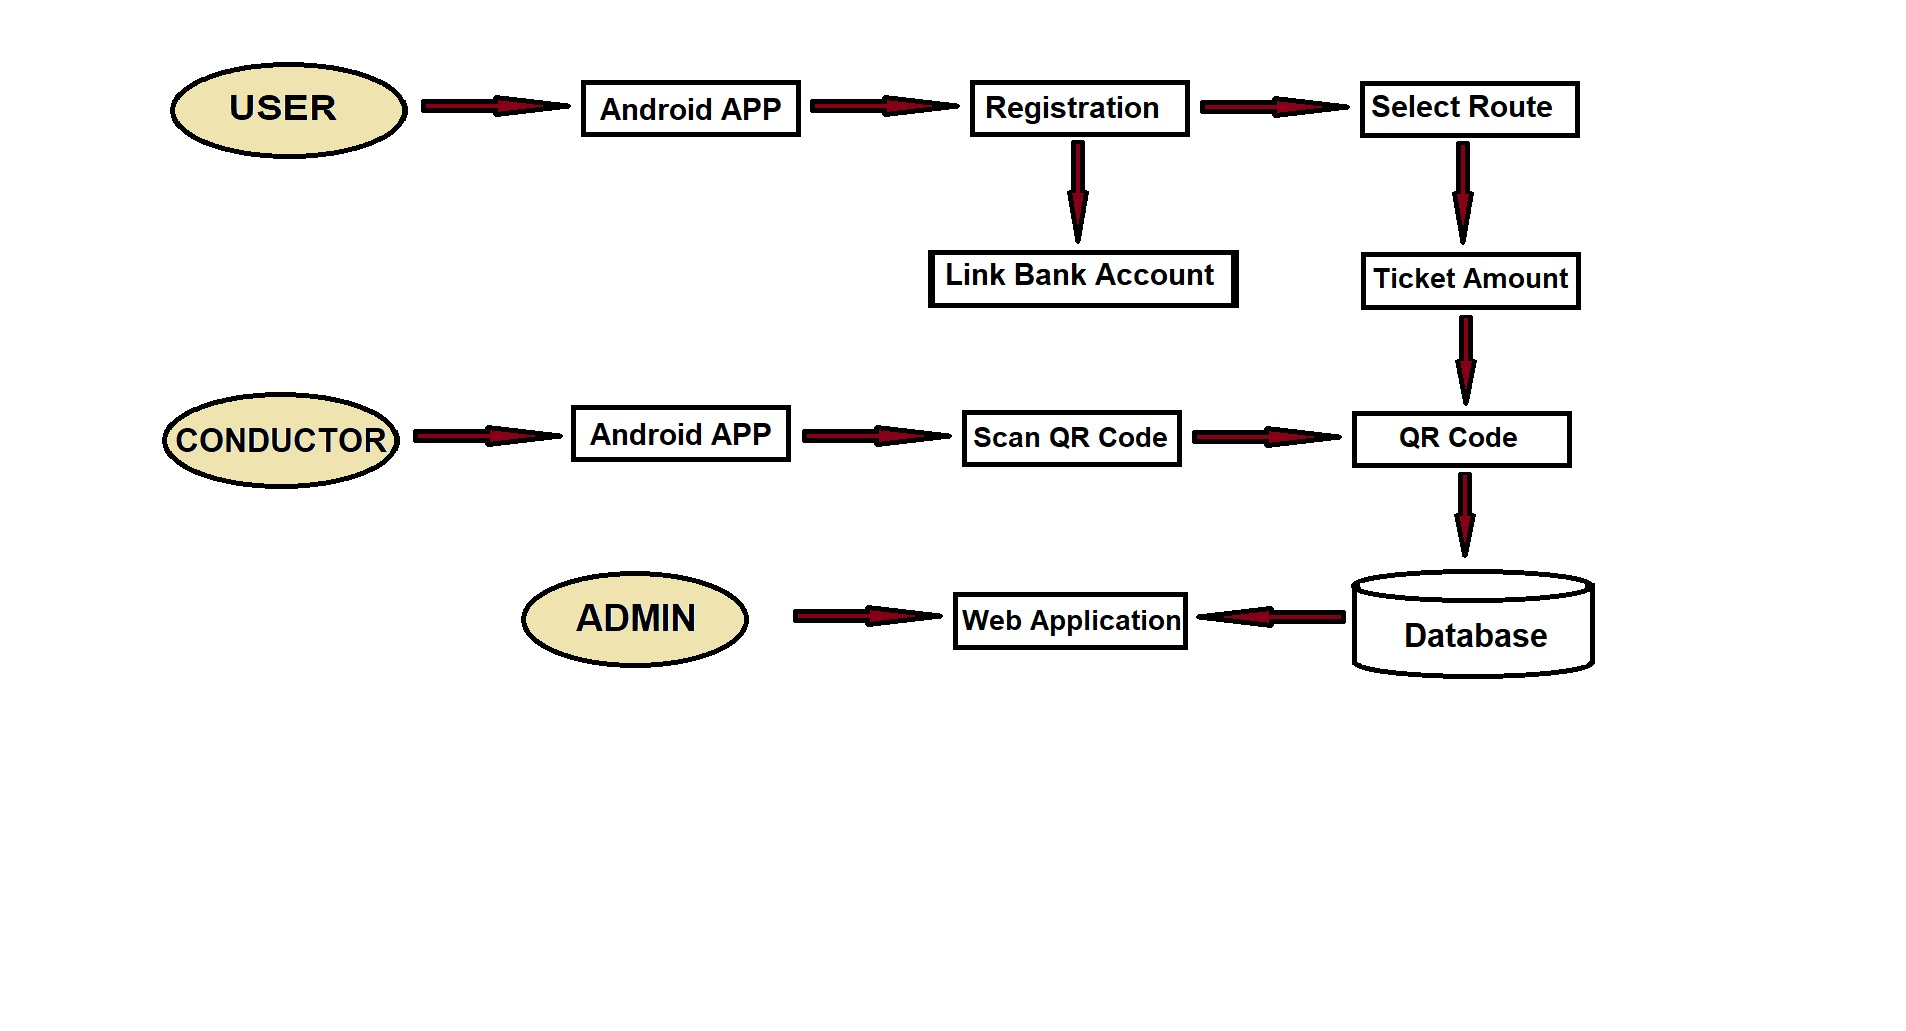
\includegraphics[width=1\textwidth]{Data FLow Diagram of System.jpg}
\caption{Data Flow Diagram Of System}
\end{figure}

\section{ETA and MQTT Module }

The device advanced on this paper objectives to minimise the ready time to board the bus, control and optimise the fleet of buses efficaciously and to offer a actual time facts of the appearance time of the bus. The inputs used are the latitude and longitude extracted from the GPS receiver of the bus. The extracted statistics from the GPS receiver is filled with extra records together with path number, registration number, timestamp and is transmitted to a MQTT broker. The latitude and longitude is processed at the hardware mapped to compute the shortest route the use of Dijkstra`s Algorithm on a predefined listing of bus stops at the path. The region of the bus is likewise up to date to a facts logger maintained in a Google spreadsheet, that acts as a cloud storage. The facts logger serves because the anciental dataset to construct the common time primarily based totally ETA prediction version. The steps of processing are completed in every module as proven withinside the structure diagram proven in Fig. 2. The outputs received after processing the facts in actual time are the ETA to the ultimate stops and the verbal exchange of the function. Based on actual time function updates, dependable facts may be given to commuters and additionally higher tracking of the fleet of buses may be completed.The glide of facts on this environment is illustrated in Fig. 3. The structure diagram and the modules of the whole device are represented in Fig. 2. The region of the bus is captured the use of a GPS receiver.

\begin{figure}
\centering
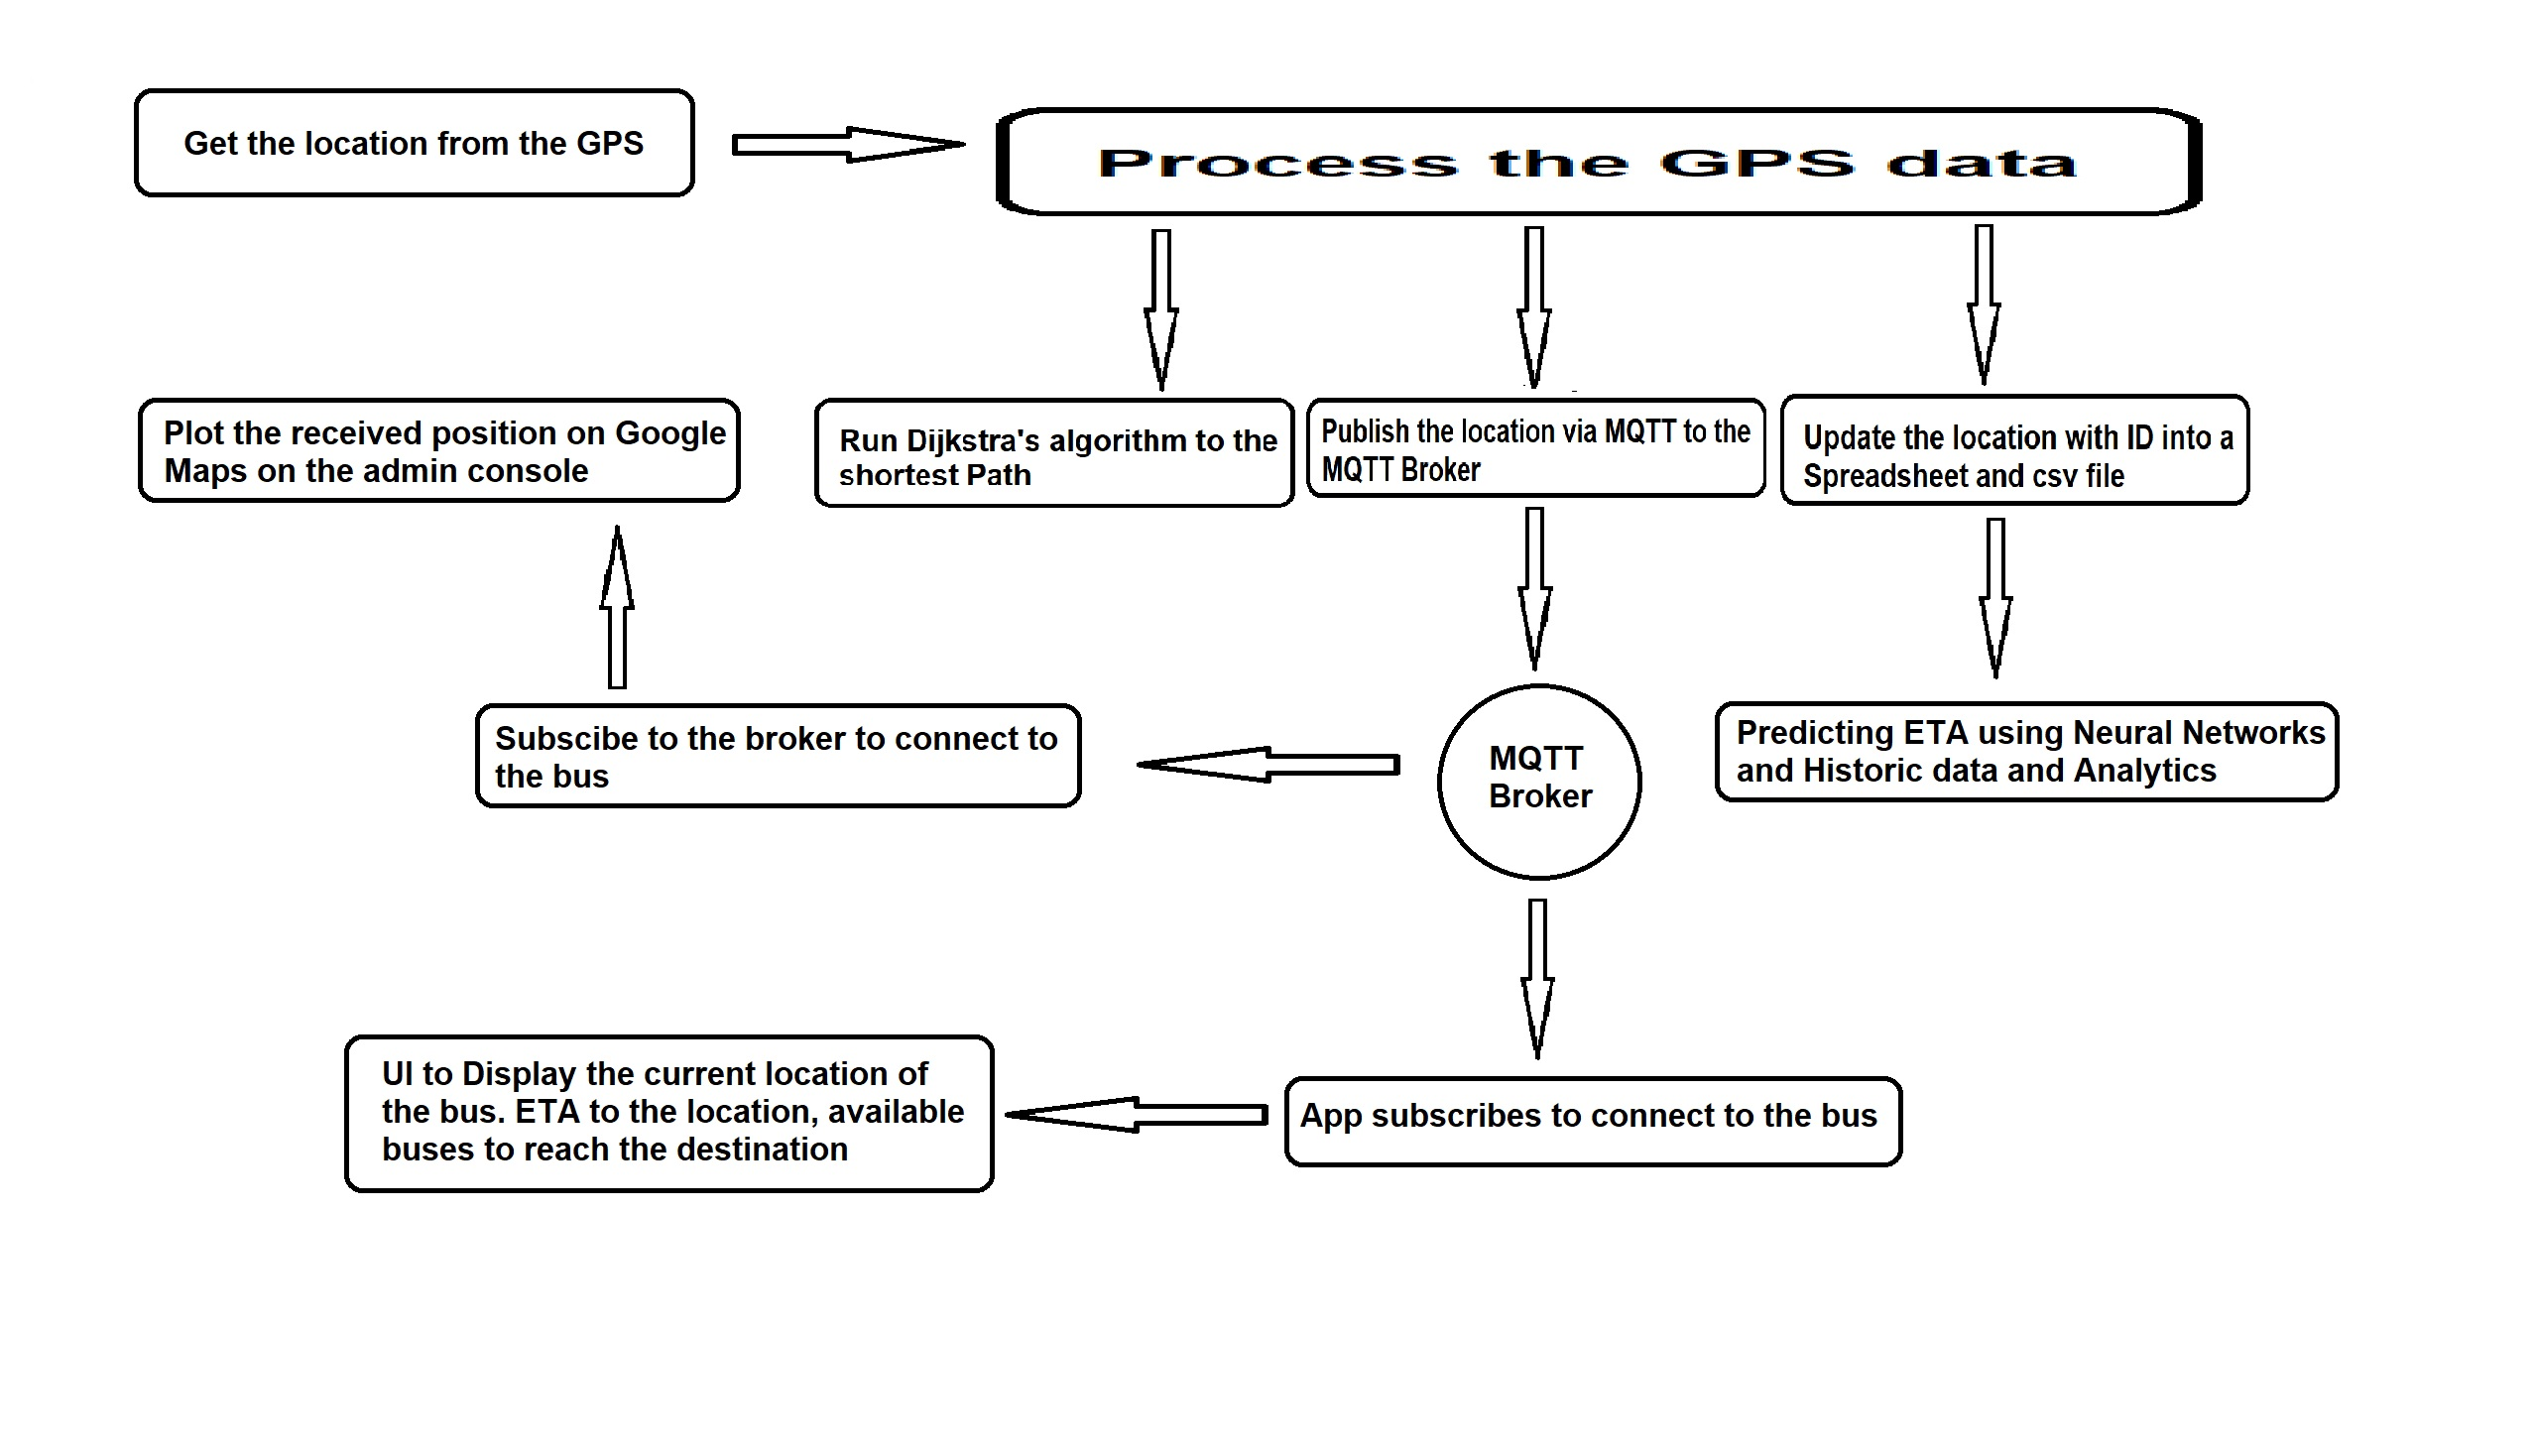
\includegraphics[width=1\textwidth]{Architecture Diagram of The System.jpg}
\caption{Architecture Diagram of The System}
\end{figure}

The data from the GPS is streamed constantly and it contains the Latitude, Longitude, Number of Satellites that the GPS receiver is capable of join to, Deviation or Error withinside the position (in phrases of metres),etc. The facts is cleaned and the Latitude and Longitude is extracted from the data stream. The latitude and longitude are the inputs to the Dijkstra`s Algorithm to compute the shortest distance to the destination (that's preset for the complete journey) from the present day position. To facilitate the capacity to file and save the motion of every bus, a data logger is designed. The information logger periodically populates a Google spreadsheet and a CSV record with the timestamp, registration number, call of the driver, destination and location of the bus. The use of Google Sheets is a cost-powerful technique and saves time putting in a custom cloud infrastructure. A csv record is maintained onboard the hardware at the bus. The cause of the csv record is to usher in redundancy to prevent data loss or data corruption and it acts just like the black box in aircraft. Each bus is related to a unique, particular subject matter (registration no.). A subject matter is the parameter in MQTT that's used to push/fetch the correct contents from the MQTT dealer. This makes certain that a quick scalability of the prototype is possible. A prediction version primarily based totally at the historic facts is constructed to estimate the appearance time of the bus to any precise stop at the route. The bus may be monitored in actual time with the aid of using the administrator the use of a easy internet application. The commuter makes use of the proposed app to get actual-time facts in regards to the modern-day region of the bus and an Estimated Arrival Time to his/her stop.The utilization sample of the proposed application is upto the user`s discretion as as soon as the app is attached to the MQTT broker the essential data could be available with the app.


\begin{figure}
\centering
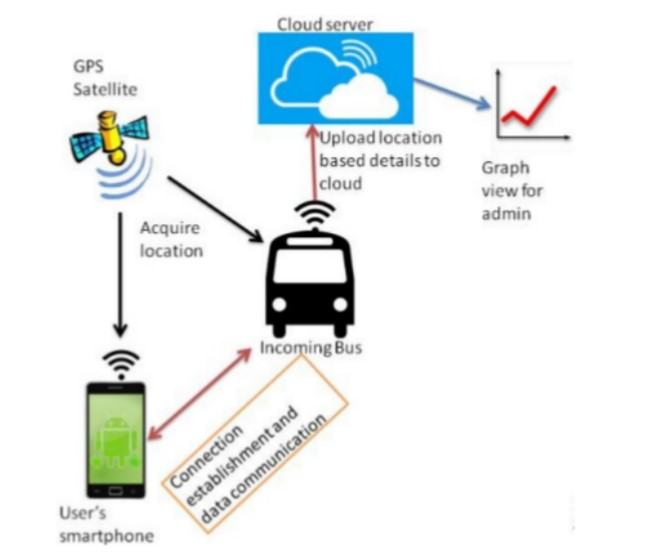
\includegraphics[width=1\textwidth]{overview.jpg}
\caption{An Overview of the data flow in the system}
\end{figure}

%\newpage

\chapter{Conclusion }
In summary, this task pursuits to present a clean ticketing experience for each conductor and passenger. The paper overcomes the issues of the transport device in an individual`s life. The device offers passengers a brand new revel in of ticketing to be able to be smooth to recognize and beneficial with the aid of using going cash- less, decreasing time for purchasing tickets and storing the information of tour of passengers. The tasks additionally make a contribution little closer to nature with the aid of using paperless transactions. Since the quantity is immediately debited from the passenger's software wallet to the conductor's software wallet, it overcomes the hassle of maintaining or returning change. The task additionally allows withinside the concept of creating virtual India.
This paper proposes a clever virtual bus pass and payment device with the aid of using the usage of android as a platform for development. The virtual bus pass system includes functions that could assist the day by day commuters of their everyday bus journey now no longer only conveniently of use, but additionally proved to be a cost-efficient technique in contrast to the traditional system. This work now no longer only contributes to the society but also to the green India marketing campaign removing the usage of paper. The paper demonstrates the usage of an android software that eases the problem of passengers journeying throughout the city. It additionally gives a secure manner of journeying. This version may be similarly changed and modified relying at the destiny wishes. Many extra modules and capabilities may be more desirable withinside the proposed version which includes pass category, extra functions of the software, user interface, payment class etc. In this fast moving developing world, the wishes of the human beings are as ever developing, and it is important to hold the era up to date that could match the present day requirements. That is why the model of this proposed version has a huge scope of change and upgradation withinside the destiny.


\titleformat{\chapter}[display]
{\centering\normalfont\huge\bfseries}
{\chaptertitlename\ \thechapter}{20pt}{\Huge}

%\prefacesection{Conclusion }
%\chapter{Conclusion}
%In summary, this task pursuits to present a clean ticketing experience for each conductor and passenger. The paper overcomes the issues of the transport device in an individual`s life. The device offers passengers a brand new revel in of ticketing to be able to be smooth to recognize and beneficial with the aid of using going cash- less, decreasing time for purchasing tickets and storing the information of tour of passengers. The tasks additionally make a contribution little closer to nature with the aid of using paperless transactions. Since the quantity is immediately debited from the passenger's software wallet to the conductor's software wallet, it overcomes the hassle of maintaining or returning change. The task additionally allows withinside the concept of creating virtual India.
This paper proposes a clever virtual bus pass and payment device with the aid of using the usage of android as a platform for development. The virtual bus pass system includes functions that could assist the day by day commuters of their everyday bus journey now no longer only conveniently of use, but additionally proved to be a cost-efficient technique in contrast to the traditional system. This work now no longer only contributes to the society but also to the green India marketing campaign removing the usage of paper. The paper demonstrates the usage of an android software that eases the problem of passengers journeying throughout the city. It additionally gives a secure manner of journeying. This version may be similarly changed and modified relying at the destiny wishes. Many extra modules and capabilities may be more desirable withinside the proposed version which includes pass category, extra functions of the software, user interface, payment class etc. In this fast moving developing world, the wishes of the human beings are as ever developing, and it is important to hold the era up to date that could match the present day requirements. That is why the model of this proposed version has a huge scope of change and upgradation withinside the destiny.

%%%%%\appendix
%\input{appendix}

%\nocite{*}
% \renewcommand{\bibname}{References}
% \bibliographystyle{IEEEtran}
% \bibliography{ref1}
\chapter{References}
% @article{viola2001rapid,
%   title={Smart E-Ticketing System for Public Transport Bus},
%   author={S. Kazi, M. Bagasrawala, F. Shaikh and A. Sayyed},
%   journal={2018 International Conference on Smart City and Emerging Technology (ICSCET), Mumbai, 2018.},
%  }

\new [1] S. Kazi, M. Bagasrawala, F. Shaikh and A. Sayyed, ”Smart E-Ticketing System for Public Transport Bus,” 2018 International Conference on Smart City and Emerging Technology (ICSCET), Mumbai, 2018. 
\new[2] Saurabh C. and Balram T. ”Public transport system ticketing system using RFID and ARM processor Perspective Mumbai bus facility B.E.S.T,” 2014 International Journal of Electronics and Computer Science Engineering ISSN- 2277- 1956, 
\new[3] S. Karthick. and A. Velmurugan., ”Android suburban railway ticketing with GPS as ticket checker,” 2012 IEEE International Conference on Advanced Communication Control and Computing Technologies (ICACCCT). 
\new[4] Shital Kotle, Korke Jayshree D., Kandharkar Snehal B., Gaikwad Pranali A. and Kale Geetanjali J., ”Smart Bus Ticketing Destination Announcement System Using QR-Code,” 11th International Conference on Recent Innovations in Science, Engineering and Management, ISBN:978-93-87793-19-4, 2018. 
\new[5] V. Malathi, B. Balamurugan and S. Eshwar, ”Achieving Privacy and Security Using QR Code by Means of Encryption Technique in ATM,” 2017 Second International Conference on Recent Trends and Challenges in Computational Models (ICRTCCM). 
\new[6] P. Telluri, S. Manam and J. M. Oli, ”Automated Bus Ticketing System Using RFID,” 2019 2nd International Conference on Intelligent Computing, Instrumentation and Control Technologies (ICICICT). 
\new[7] V. Ceronmani Sharmila, S. Monesh, R. Aayush, G. Karesh and I.Ibrahim, ”Digitized Bus Ticketing Framework,” 2019 1st International Conference on Innovations in Information and Communication Technology (ICIICT). 
\new[8] K. Hargunani, P. Kengar, M. Lokhande, R. Gawade and S. K. More,”Integrated Bus System Using QR Code,” 2018 Fourth International Conference on Computing Communication Control and Automation (ICCUBEA). 
\new[9] R. B. Torode, ”Prestige-contactless smartcard ticketing on London Transport,” 1996 International Conference on Public Transport Electronic Systems (Conf. Publ. No. 425), London, UK, 1996. 
\new[10] M. Arora, C. Kumar and A. K. Verma, ”Increase Capacity of QR Code Using Compression Technique,” 2018 3rd International Conference and Workshops on Recent Advances and Innovations in Engineering (ICRAIE)



% @misc{bworld,
%   author = {Ingo Lütkebohle},
%   title = {{BWorld Robot Control Software}},
%   howpublished = "\url{http://aiweb.techfak.uni-bielefeld.de/content/bworld-robot-control-software/}",
%   year = {2008}, 
%   note = "[Online; accessed 19-July-2008]"
% }


\titleformat{\chapter}[display]
{\centering\normalfont\huge\bfseries}
{\chaptertitlename\ \thechapter}{20pt}{\Huge}

\chapter{Report Documentation}

\begin{table}
\begin{center}
\begin{tabular}{|c|} \hline 
Report Documentation\\ \hline
Report code : CS-TE-Seminar 2022-23 \\		\hline
Report Number : 55 \\ 		\hline
Address (Details) : \\
SNJB’s Late Sau. Kantabai Bhavarlalji Jain College of Engineering,\\ Jain Gurukul, Neminagar, Chandwad, Nashik, Pin Code - 423 101, Maharashtra, India \\ \hline		
Author     : Sagar Ganesh Sharma \\
Address   : Ganesh Nagar, Near Satsang Bhavan, Manmad - 423 104, \\ Dist. : Nashik, Maharashtra, India \\
Email       : er.sagargsharma@gmail.com \\
Roll No.   : 55 \\
Mob. No. : 9960726868
\\ 	\hline	
Academic Year : 2022-2023 \\
Branch : Computer Engineering
\\ 		\hline

Key Words : Smart, Bus, System, Passenger, Conductor, Database, \\ Public transport, Bus tickets, Android application, QR Code, IoT, \\ Smart Bus, Smart Cities, MQTT, Estimated Time of Arrival (ETA), \\ Dynamic Shortest Path, Dijkstra’s Algorithm \\ 		\hline
\begin{tabular}{|p{3.3cm}|p{3cm}|p{3cm}|p{3cm}|p{3cm}|}
 Type of Report : FINAL & Report Checked By :    & Report Checked Date : & Guides Complete Name : 
Prof. Yogita K. Desai & Total Copies  : 2
\\\end{tabular} \\ \hline
\begin{tabular}{|p{15cm}|}
 Abstract : \\
Public transport is the cheapest and most reliable transportation system in India,\\ hence it has always been popular with the masses. Buses are an integral means of public trans- port which plays a vital role in transportation in India. The advancement in the transport system has been increasing in day-to- day life as more and more people rely on public transport to go to work, school, hospitals, etc. Even though the public transport buses have been providing fairly satisfactory services, there is a need for a smart and reliable system. The major problem in local buses are about issuing bus tickets, which often leads to conflict between the passenger and the conductor. Keeping this in mind we are developing an android application which will provide an efficient and smooth bus ticketing experience for both the user(passenger) and the service provider(conductor). The android application provides an interface for the bus ticketing system combined with the technology of QR Code for quick money transfer. QR Code or the Quick Response Code is the most dominant form of storing and exchanging information between devices. It’s a type of matrix BarCode and has more capacity than UPC Codes. Typically scanned and interpreted by a camera enabled smartphone, but also can be interpreted or generated by any camera device implemented with QR decoding logic. The passengers can go cashless using this application, and the conductor does not have to worry about returning change for the paid bus fare. By this application, we can minimise the usage of paper tickets which will also help in green India. 
\\\end{tabular} \\ \hline
  \end{tabular}
   \end{center}
\end{table}





%Use following command at the command prompt to display the Index
% makeindex thesis
%%%%%\newpage
%%%%%\addcontentsline{toc}{chapter}{Index}
%%%%%\printindex

\end{document}
